\section{Compartilhamento público}
\label{s.public_sharing}

\begin{frame}{Compartilhamento público}
	\justify
	\begin{itemize}
		\item<1> Qualquer tipo de \textbf{compartilhamento}, que não fira direitos coletivos/individuais e que seja \textbf{benéfico} para a sociedade, é extremamente \textbf{bem-vindo};
		\\~\\
		\item<2> O compartilhamento público permite o \textbf{desenvolvimento} da sociedade, principalmente na área de \textbf{tecnologia};
	\end{itemize}
\end{frame}

\subsection{Pré-publicação}
\label{ss.preprint}

\begin{frame}{Pré-publicação}
	\justify
	\begin{itemize}
		\item<1> \textbf{Manuscritos} hospedados em servidores \textbf{públicos} prévios à publicação;
		\\~\\
		\item<2> A \textbf{utilização} deve ser \textbf{cautelosa} pois ainda não foi submetido à revisão por pares (\emph{peer review});
		\\~\\
		\item<3> Entretanto, trazem benefícios, tais como, \textbf{visibilidade}, evidência de \textbf{produtividade}, \textbf{acessibilidade} e \textbf{agilidade}.
	\end{itemize}
\end{frame}

\begin{frame}{}
	\begin{figure}
		\centering
		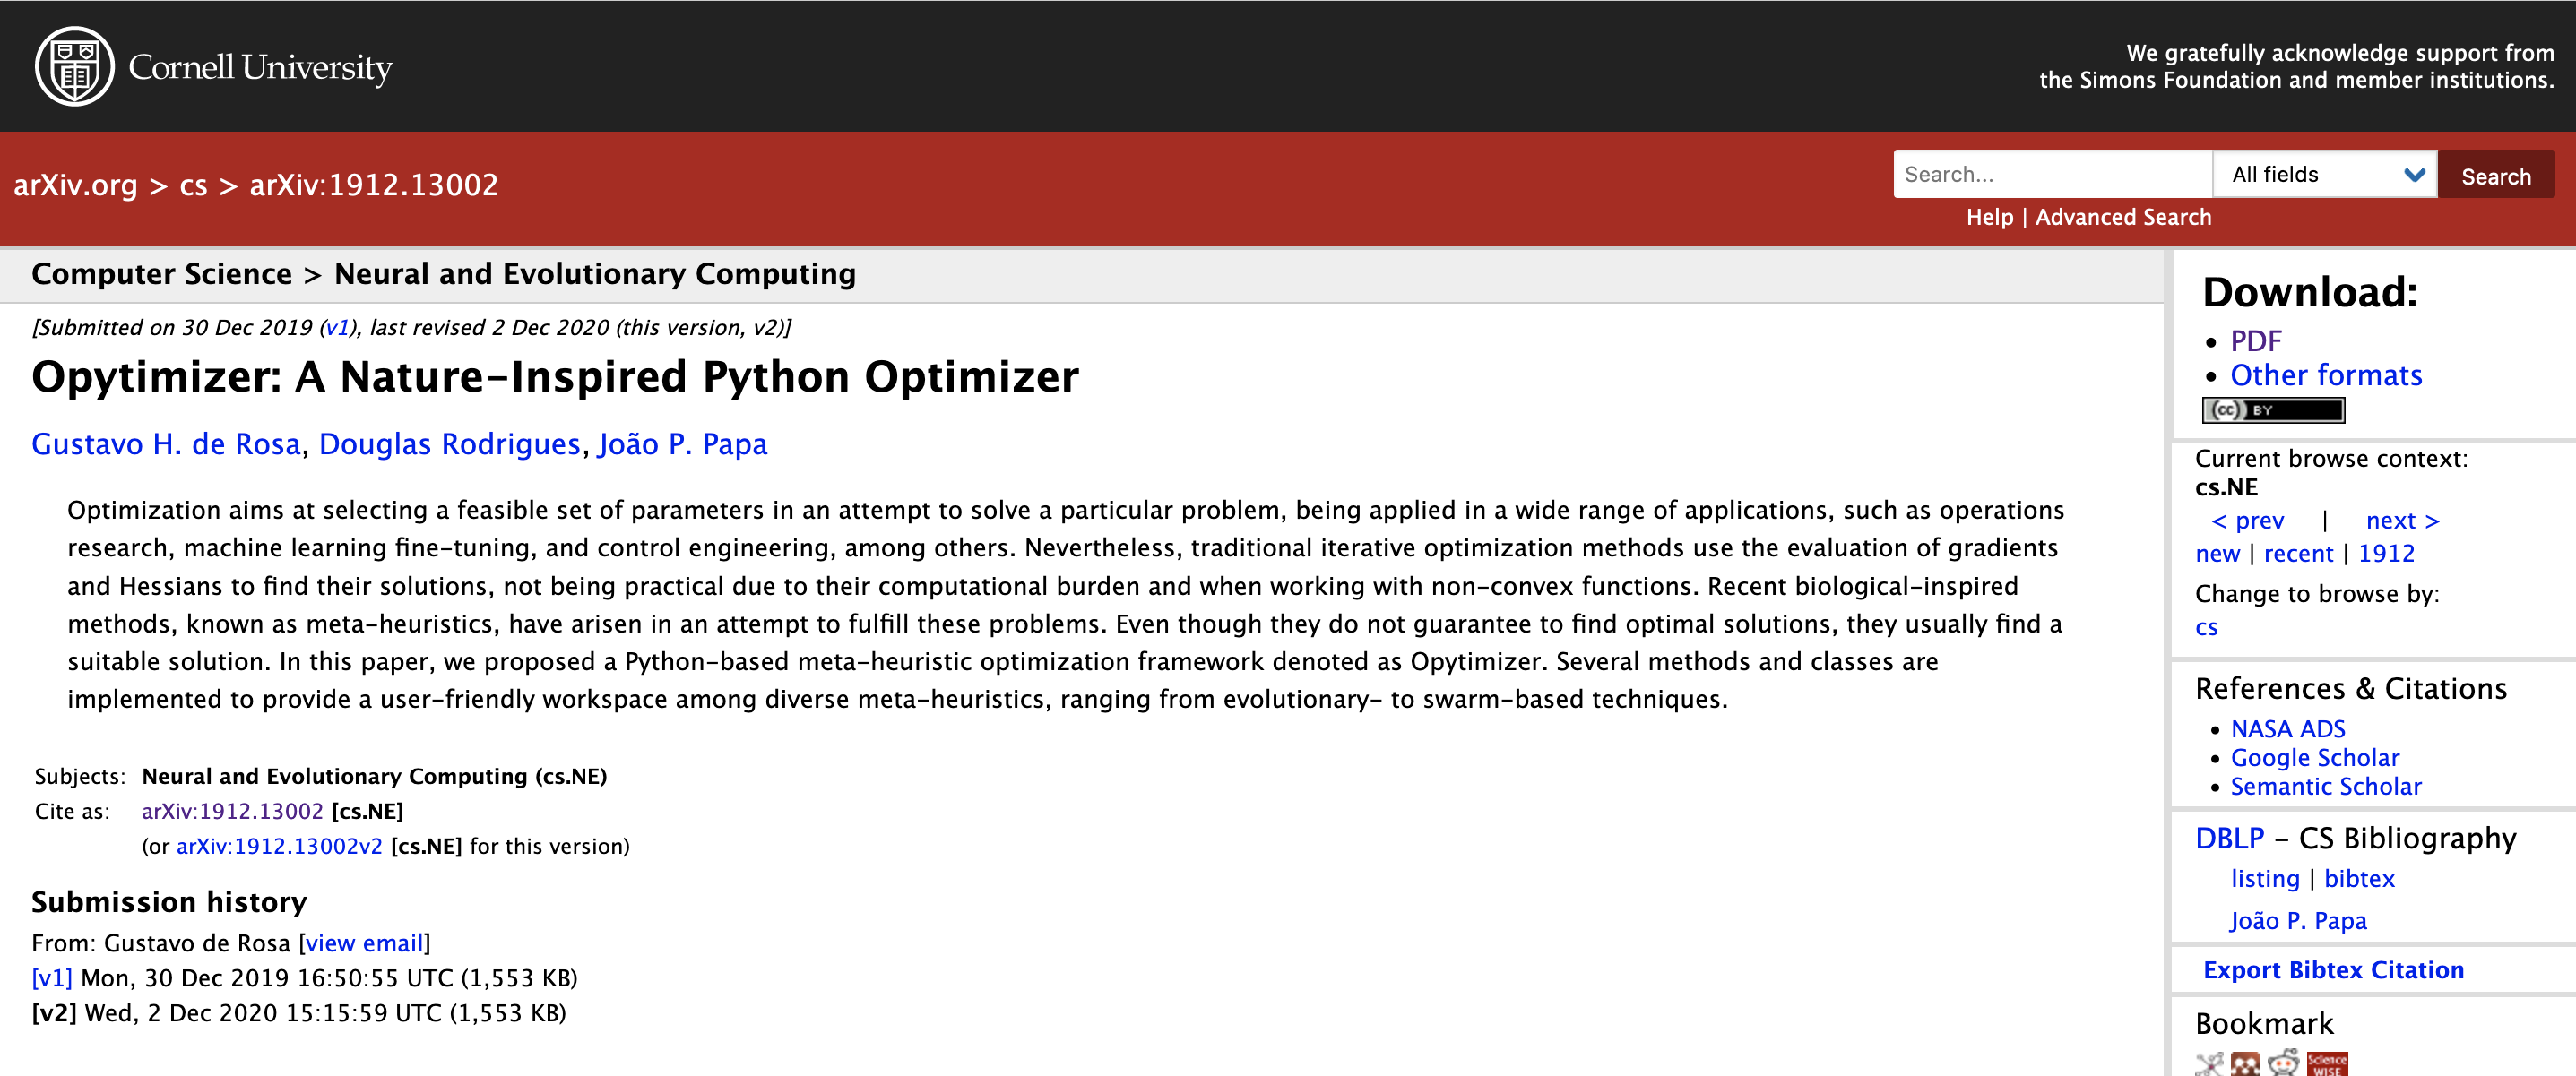
\includegraphics[scale=0.215]{figs/arxiv_paper.png}
		\caption{Exemplo de  manuscrito hospedado no arXiv e acessível por qualquer pessoa: \url{https://arxiv.org/pdf/1912.13002.pdf}.}
		\label{f.arxiv_paper}
	\end{figure}
\end{frame}

\subsection{Código aberto}
\label{ss.open_source}

\begin{frame}{Código aberto}
	\begin{figure}
		\centering
		
\includegraphics[scale=0.425]{figs/open_source_word_cloud.png}
		\caption{Nuvem de palavras relacionadas ao \emph{open-source} (código aberto)~\cite{Silva:21}.}
		\label{f.open_source_word_cloud}
	\end{figure}
\end{frame}

\begin{frame}{}
	\begin{figure}
		\centering
		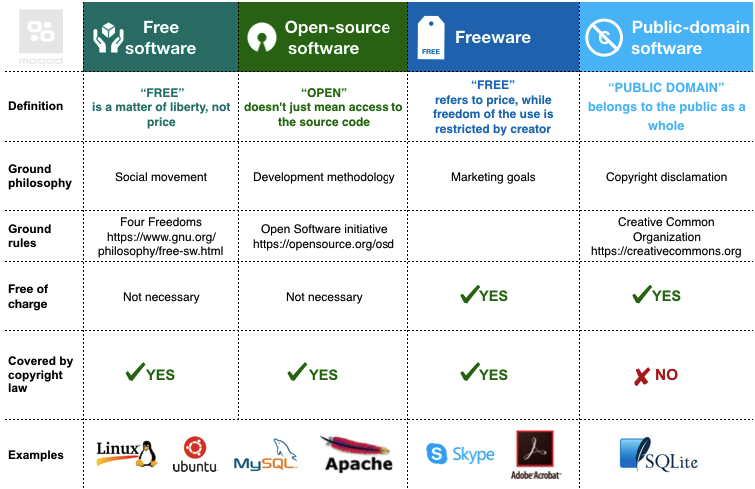
\includegraphics[scale=0.35]{figs/open_source_difference.png}
		\caption{Quadro comparativo entre \emph{software} livre, de código aberto, gratuito e de domínio público~\cite{Todavchich:21}.}
		\label{f.open_source_difference}
	\end{figure}
\end{frame}

\begin{frame}{}
	\begin{figure}
		\centering
		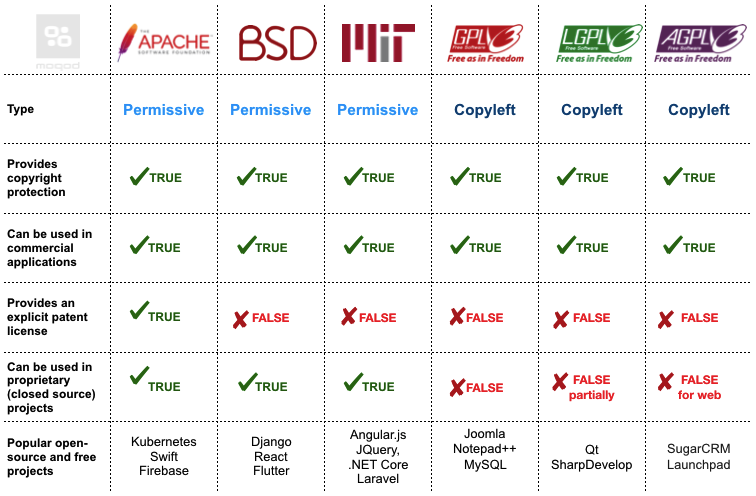
\includegraphics[scale=0.325]{figs/open_source_license.png}
		\caption{Quadro comparativo entre licenças amplamente utilizadas em projetos de código aberto~\cite{Todavchich:21}.}
		\label{f.open_source_license}
	\end{figure}
\end{frame}

\subsection{Ferramentas gratuitas}
\label{ss.free_tools}


\begin{frame}{Ferramentas gratuitas}
	\justify 
	\begin{itemize}
		\item<1> \textbf{Repositório de pré-publicação}: RePEc, OSF Preprints, \underline{arXiV}, SSRN, HAL, Zenodo, bioRxiv, etc;
		\\~\\
		\item<2> \textbf{Controle de versão} (protocolo \texttt{git}): \underline{GitHub}, GitLab, Bitbucket, etc;
		\\~\\
		\item<3> \textbf{Gerenciamento de pacote}: .NET/Windows (NuGet), JavaScript/Node.js (npm e yarn), \underline{Python (PyPI)}, etc;
	\end{itemize}
\end{frame}